% !TeX TS-program = xelatex

\documentclass[aspectratio=169]{beamer}

\usepackage{xltxtra}
\usepackage[main=russian,english]{babel}
\defaultfontfeatures{Mapping=tex-text}
\usepackage{listings}
\usepackage[export]{adjustbox}

\usepackage[backend=biber,bibstyle=numeric,citestyle=numeric-comp,sorting=none,defernumbers=true,date=long]{biblatex}
\addbibresource{dns-security.bib}

\usetheme{shl2021}

% for biblatex
\setbeamerfont{bibliography item}{size*={8pt}{1}}
\setbeamertemplate{bibliography item}{\insertbiblabel}
\renewcommand*{\bibfont}{\clbr\fontsize{8}{8}\selectfont}
\DeclareFieldFormat{url}{\color{blue}\url{#1}}

% for listings
% Solarized colors
\definecolor{sbase03}{HTML}{002B36}
\definecolor{sbase02}{HTML}{073642}
\definecolor{sbase01}{HTML}{586E75}
\definecolor{sbase00}{HTML}{657B83}
\definecolor{sbase0}{HTML}{839496}
\definecolor{sbase1}{HTML}{93A1A1}
\definecolor{sbase2}{HTML}{EEE8D5}
\definecolor{sbase3}{HTML}{FDF6E3}
\definecolor{syellow}{HTML}{B58900}
\definecolor{sorange}{HTML}{CB4B16}
\definecolor{sred}{HTML}{DC322F}
\definecolor{smagenta}{HTML}{D33682}
\definecolor{sviolet}{HTML}{6C71C4}
\definecolor{sblue}{HTML}{268BD2}
\definecolor{scyan}{HTML}{2AA198}
\definecolor{sgreen}{HTML}{859900}
\lstset{
        columns=flexible,
        keepspaces=true,
        showstringspaces=false,
        showtabs=false,
        tabsize=4,
        frame=single,
        basicstyle=\fontsize{10pt}{12}\ttfamily\color{sbase00},
        backgroundcolor=\color{sbase3},
        keywordstyle=\color{scyan},
        commentstyle=\color{sbase1},
        stringstyle=\color{sblue},
        numberstyle=\color{sviolet},
        identifierstyle=\color{sbase00},
        rulecolor=\color{sbase1},
        framerule=1pt
}

\lstdefinelanguage{nginx}{
        morestring=[b]{"},
        morecomment=[l]\#,
        morekeywords={map,default,server,listen,proxy_pass,ssl_preread,on}
}

% for listings background
\makeatletter
\let\old@lstKV@SwitchCases\lstKV@SwitchCases
\def\lstKV@SwitchCases#1#2#3{}
\makeatother
\usepackage{lstlinebgrd}
\makeatletter
\let\lstKV@SwitchCases\old@lstKV@SwitchCases

\lst@Key{numbers}{none}{%
    \def\lst@PlaceNumber{\lst@linebgrd}%
    \lstKV@SwitchCases{#1}%
    {none:\\%
     left:\def\lst@PlaceNumber{\llap{\normalfont
                \lst@numberstyle{\thelstnumber}\kern\lst@numbersep}\lst@linebgrd}\\%
     right:\def\lst@PlaceNumber{\rlap{\normalfont
                \kern\linewidth \kern\lst@numbersep
                \lst@numberstyle{\thelstnumber}}\lst@linebgrd}%
    }{\PackageError{Listings}{Numbers #1 unknown}\@ehc}}
\makeatother

\makeatletter
%%%%%%%%%%%%%%%%%%%%%%%%%%%%%%%%%%%%%%%%%%%%%%%%%%%%%%%%%%%%%%%%%%%%%%%%%%%%%%
%
% \btIfInRange{number}{range list}{TRUE}{FALSE}
%
% Test in int number <number> is element of a (comma separated) list of ranges
% (such as: {1,3-5,7,10-12,14}) and processes <TRUE> or <FALSE> respectively

\newcount\bt@rangea
\newcount\bt@rangeb

\newcommand\btIfInRange[2]{%
    \global\let\bt@inrange\@secondoftwo%
    \edef\bt@rangelist{#2}%
    \foreach \range in \bt@rangelist {%
        \afterassignment\bt@getrangeb%
        \bt@rangea=0\range\relax%
        \pgfmathtruncatemacro\result{ ( #1 >= \bt@rangea) && (#1 <= \bt@rangeb) }%
        \ifnum\result=1\relax%
            \breakforeach%
            \global\let\bt@inrange\@firstoftwo%
        \fi%
    }%
    \bt@inrange%
}
\newcommand\bt@getrangeb{%
    \@ifnextchar\relax%
        {\bt@rangeb=\bt@rangea}%
        {\@getrangeb}%
}
\def\@getrangeb-#1\relax{%
    \ifx\relax#1\relax%
        \bt@rangeb=100000%   \maxdimen is too large for pgfmath
    \else%
        \bt@rangeb=#1\relax%
    \fi%
}

%%%%%%%%%%%%%%%%%%%%%%%%%%%%%%%%%%%%%%%%%%%%%%%%%%%%%%%%%%%%%%%%%%%%%%%%%%%%%%
%
% \btLstHL<overlay spec>{range list}
%
% TODO BUG: \btLstHL commands can not yet be accumulated if more than one overlay spec match.
% 
\newcommand<>{\btLstHL}[1]{%
\only#2{\btIfInRange{\value{lstnumber}}{#1}{\color{sbase2}\def\lst@linebgrdcmd{\color@block}}{\def\lst@linebgrdcmd####1####2####3{}}}%
}%
\makeatother

\title{Безопасность DNS}
\author{Филипп Кулин}

\begin{document}

\begin{frame}
\titlepage
\end{frame}

\begin{frame}{Откиньтесь на спинку кресла}
        \begin{itemize}
                \item Эта презентация сделана с помощью \LaTeX
                \item Я расскажу страшную сказку
                \item Тема DNS очень специфична % мало кто лезет под капот, а кто лезет - быстро забывает %\item Я сделаю акцент на эксплуатацию сервисов
        \end{itemize}
        Пока я тут болтаю, вы можете поставить вот такие вот программы
\end{frame}

\begin{frame}{DNS --- всему голова}
        \begin{itemize}
                \item Жизнь пользователей в сети
                \item Запросы к API, работа с CDN
                \item Облака, микросервисы, автообнаружение и конфигурация
                \item Невообразимое количество всего
        \end{itemize}
\end{frame}

\begin{frame}{Тайная жизнь привычных программ}
% Мои любимые примеры
        \begin{itemize}
                \item<1-> SSHD определяет домен для подключившегося IP\\{\small и этот факт является одним из источников седых волос у админов}
                \item<2-> MySQL определяет домен для подключившегося IP
                \item<3-> Apache определяет домен для подключившегося IP\\{\small даже если \texttt{HostnameLookups Off}, но есть \texttt{Require}}
                \item<4-> Microsoft Windows постоянно шлет DNS Update в сеть
                \item<5-> Docker, Kubernetes, etc
                \item<6-> \textbf{Запустите tcpdump/WireShark}
        \end{itemize}
\end{frame}

\begin{frame}{DNS --- это просто?}
        Три каверзных вопроса:
        \begin{itemize}
                \item<1-> Каков максимальный размер доменного имени? % Паскалевские строки с длиной в начале и 63 символами, последняя длина 0, всё вместе 255
                \item<2-> Точку на конце надо ставить? % 1. Это удобно программам 2. Их этого произошли правила интерпретации
                \item<3-> Что именно спрашивает ресолвер и что отвечают DNS-сервера при рекурсивном обходе?
        \end{itemize}
        % во время подготовки к докладу я нашел ошибку/неточность в сервере NSD
\end{frame}

\begin{frame}[t]{Как устроен DNS}%
        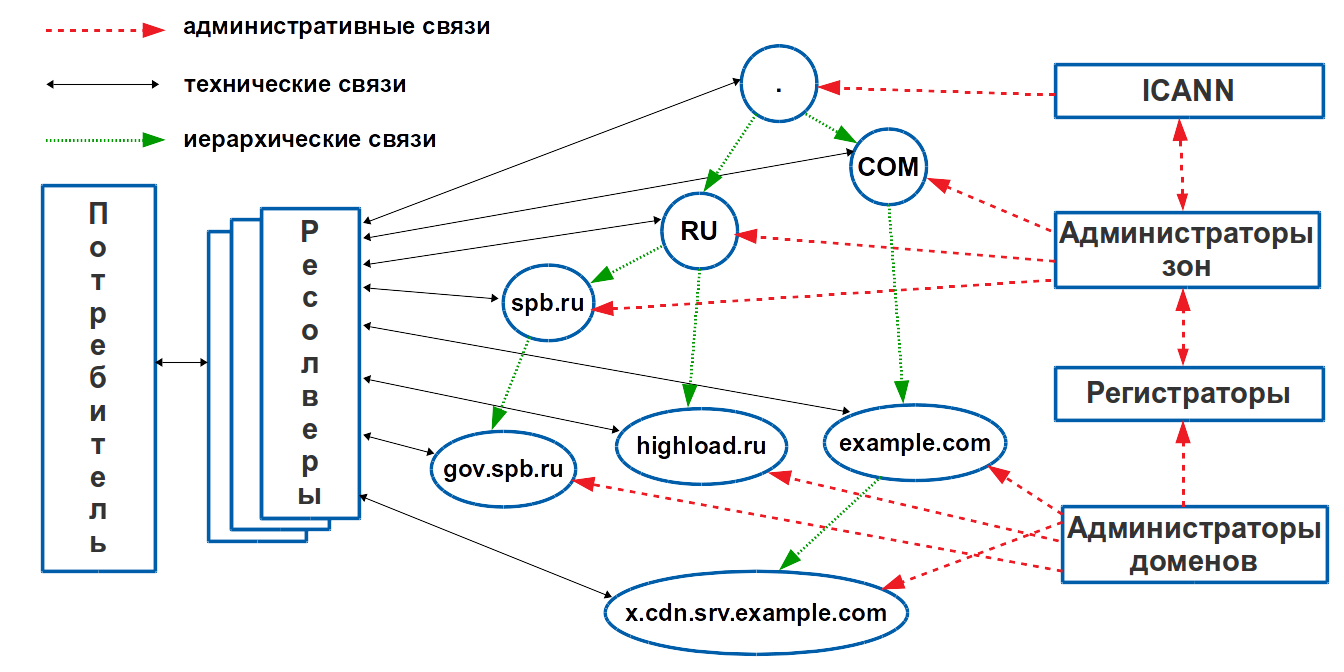
\includegraphics[height=0.8\textheight]{pic1.png}
\end{frame}

\begin{frame}{Особенности классического DNS}
        \begin{itemize}
                \item UDP транспорт. Нет соединения
                \item Нет идентификации серверов DNS
                \item Нет контроля данных
                \item Нет шифрования
        \end{itemize}
\end{frame}

\begin{frame}{Угорозы в системе DNS}
        \centering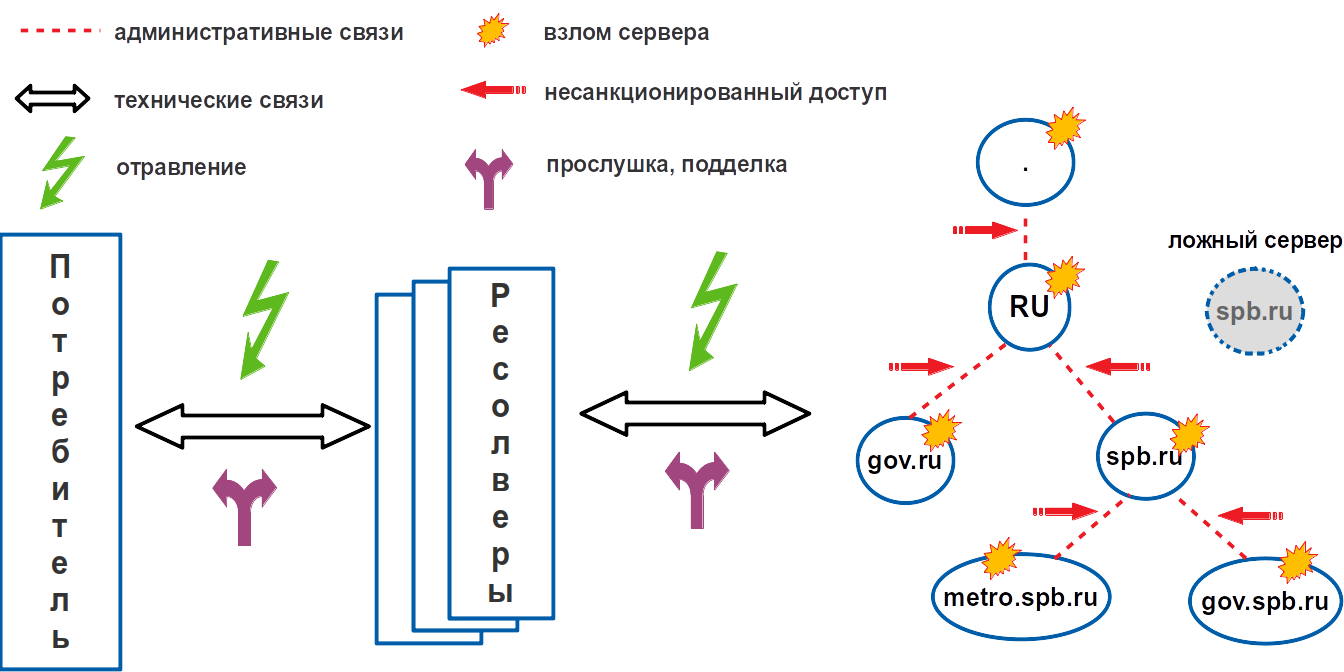
\includegraphics[height=0.75\textheight]{pic2.png}
\end{frame}

\begin{frame}{Заложенная в DNS безопасность}
        \onslide<2->{``... действия, которые с современной точки зрения могут показаться неправильными или ошибочными,
        часто оказывались естественным следствием господствовавшего в те времена понимания тех или иных вещей, а
        также ограниченности доступных ресурсов.``}
        \onslide<3-> \rightline{{\rm --- Брайан Керниган}}\supercite{unix-memoir}
\end{frame}

% завидую хакерам 80-ых и 90-ых - халява

% https://en.wikipedia.org/wiki/DNS_hijacking
% A number of consumer ISPs such as AT&T,[4] Cablevision's Optimum Online,[5] CenturyLink,[6] Cox Communications, RCN,[7] Rogers,[8] Charter Communications (Spectrum), Plusnet,[9] Verizon,[10] Sprint,[11] T-Mobile US,[12] Virgin Media,[13][14] Frontier Communications, Bell Sympatico,[15] Deutsche Telekom AG,[16] Optus,[17] Mediacom,[18] ONO,[19] TalkTalk,[20] Bigpond (Telstra),[21][22][23][24] TTNET, Türksat, and Telkom Indonesia[25] use or used DNS hijacking for their own purposes, such as displaying advertisements[26] or collecting statistics. Dutch ISPs XS4ALL and Ziggo use DNS hijacking by court order: they were ordered to block access to The Pirate Bay and display a warning page instead.[27] These practices violate the RFC standard for DNS (NXDOMAIN) responses,[28] and can potentially open users to cross-site scripting attacks.[26]

% офигенно
% https://www.internetsociety.org/blog/2018/04/amazons-route-53-bgp-hijack/


% https://www.trendmicro.com/vinfo/us/security/news/cyber-attacks/hacked-or-spoofed-digging-into-the-malaysia-airlines-website-compromise

\begin{frame}{Основные проблемы}
        \begin{itemize}
                \item Подделка
                \item Прослушка
        \end{itemize}
\end{frame}

\begin{frame}{Основные проблемы. Подделка}
        \begin{itemize}
                \item<1-> Отравление
                \item<1-> Подмена
                \item<1-> Взлом серверов и замена записей
                \item<1-> Поддельные серверы, BGP-injection
                \begin{itemize}
                        \item<2-> Атака на Route53 в апреле 2018 года % https://www.internetsociety.org/blog/2018/04/amazons-route-53-bgp-hijack/
                \end{itemize}
                \item<3-> Госрегулирование
                \begin{itemize}
                        \item<3-> Блокировка сайтов в Европе и России
                \end{itemize}
        \end{itemize}
\end{frame}

\begin{frame}{Основные проблемы. Прослушка}
        \begin{itemize}
                \item<1-> Маркетинговые исследования
                \item<1-> Шпионаж и промышленный шпионаж
                \begin{itemize}
                        \item<2-> ... с использованием госрегулирования
                \end{itemize}
                \item<1-> RFC7626 -- 73.1\% могут быть узнаны по слепку DNS
                \item<2-> Госрегулирование
                \begin{itemize}
                        \item<2-> Использование DoH/DoT Telegram
                \end{itemize}
        \end{itemize}
\end{frame}

\begin{frame}{А так ли страшен чёрт?}
        \begin{itemize}
                \item<2-> DNS-уязвимости не самоцель, часто нужны условия
                \item<3-> Однако DNS никогда не в одиночестве
                \item<4-> Ваш сетевой периметр защищен? Точно?
                \item<5-> Ваша сеть получает подписанные маршруты?
                        \begin{itemize}
                                \item<6-> Вы ведете журнал странных анонсов?
                        \end{itemize}
                \item<6-> Ваши сервисы проверяют сертификат соединения? % при обращении наружу, журнал этого есть?
                \item<7-> \textbf{Однако, современные взломы чаще основаны на бардаке}
        \end{itemize}
\end{frame}

\begin{frame}{Защита от подделки}
        \begin{itemize}
                \item Не «взлетевший» DNSCurve
                \item Расширение DNSSEC
        \end{itemize}
\end{frame}

\begin{frame}{DNSCurve}
                Концепция
                \begin{itemize}
                        \item Аутентификация авторитативного DNS-сервера
                        \item Защита обмена между ресолвером и авторитативным сервером
                \end{itemize}
                Принцип действия
                \begin{itemize}
                        \item Публичный ключ DNS-сервера с магическим префиксом \texttt{"uz5"} в NS-записи домена:\\
                                {\small\texttt{\textbf{uz5}qry75vfy162c239jgx7v2knkwb01g3d04qd4379s6mtcx2f0828.dnscurve.io}}
                        \item Обмен с DNS-сервером шифруется
                \end{itemize}
\end{frame}

\begin{frame}{DNSCurve. Особенности}
        \begin{itemize}
                \item Не меняет саму спецификацию DNS
                \item Основан на вере в целостность системы
                \item Зависит от источника ответа
                \item Внедрение практически отсутствует
                \item Шифрование на основе ED25519 % кривые Эдвардса
        \end{itemize}
\end{frame}

\begin{frame}{DNSSEC}
        \begin{itemize}
                \item Концепция
                \begin{itemize}
                        \item Источник записи не важен. Используя доверенный корневой ключ, возможно проверить любую подписанную запись
                \end{itemize}
                \item Принцип действия
                \begin{itemize}
                        \item Записи зоны подписаны ключом зоны %важно - не сервера
                        \item Подтверждения подписи выстраиваются в цепочку доверия
                \end{itemize}
        \end{itemize}
\end{frame}

\begin{frame}{DNSSEC. Принцип действия}
        \begin{columns}[T,onlytextwidth]
                \begin{column}{0.5\textwidth}<1->
                        \textbf{Подпись зоны}
                        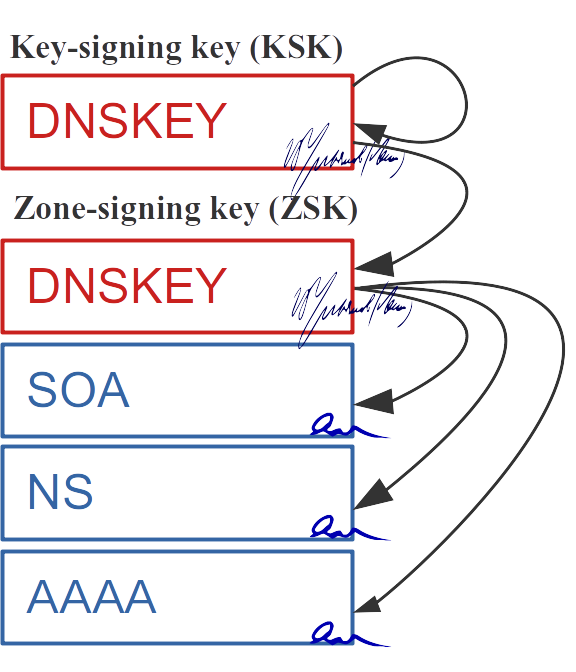
\includegraphics[height=0.7\textheight]{pic3.png}
                \end{column}
                \begin{column}{0.5\textwidth}<2->
                        \textbf{Цепочка доверия}
                        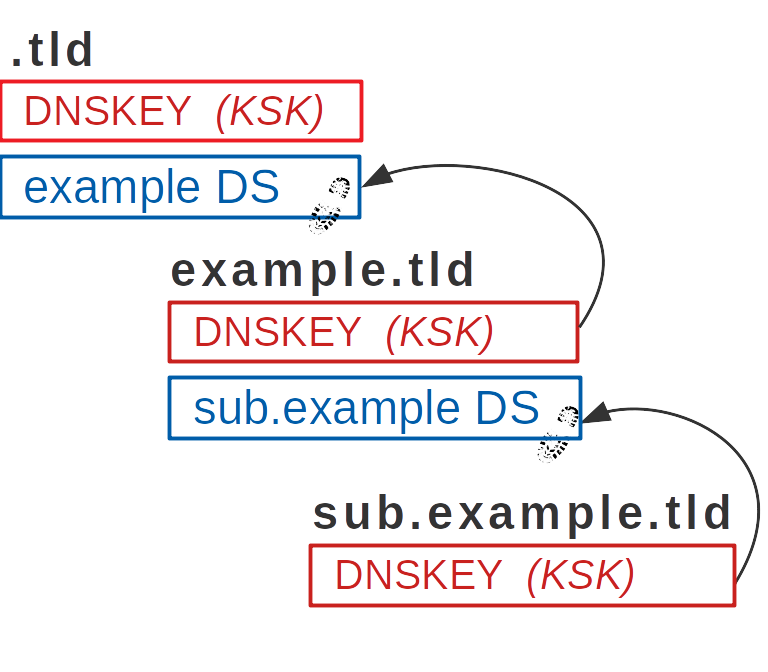
\includegraphics[height=0.7\textheight]{pic4.png}
                \end{column}
        \end{columns}
\end{frame}

\begin{frame}{DNSSEC. Особенности}
        \begin{itemize}
                \item \textbf{Источник ответа не важен}
                \item Требует аккуратности и непрерывного обслуживания даже в статическом состоянии
                \item Сложные реализации «отрицательного ответа»
                \item Большой размер ответа
                \item Возможность использования «устаревших» ответов % в рамках срока действия подписи
                \item Крайне слабая глубина внедрения
        \end{itemize}
\end{frame}

\begin{frame}{DNSSEC. Варианты использования}
        \begin{itemize}
                \item Прозрачная проверка\\
                {\small Потребитель получает фильтрованные ответы }
                \item Явная проверка\\
                {\small Потребитель явно указывает ресолверу, что хочет получить проверенный результат. Проверяет флаги ответа }
                \item Усиленная проверка\\
                {\small Потребитель проверяет подписи сам }
        \end{itemize}
\end{frame}

\begin{frame}{DNSSEC. Тренды}
        \begin{itemize}
                \item Алгоритм ECDSA
                \begin{itemize}
                        \item скорость
                        \item небольшой размер ответов по сравнению с RSA
                \end{itemize}
                \item Подпись «на лету»
                \begin{itemize}
                        \item использование «белой лжи» \supercite{dnssec-wl}
                        \item использование «чёрной лжи» \supercite{dnssec-bl}
                \end{itemize}
        \end{itemize}
\end{frame}

\begin{frame}{DNSSEC. Поддержка}        
СКОРЕЕ ВСЕГО ЗАМЕНЮ ОБЗОРОМ "КАК ПОСМОТРЕТЬ"
        \begin{itemize}
                \item \textbf{Клиенты} \\
                \texttt{dig/delv, drill, kdig}
                \item \textbf{Ресолверы} \\
                \texttt{systemd-resolved, dnsmask, unbound, KNOT Resolver, CoreDNS, PowerDNS recursor, BIND}
                \item \textbf{Авторитативные сервера DNS} \\
                \texttt{KNOT, CoreDNS, PowerDNS, NSD, YADIFA, BIND}
                \item \textbf{Сервера DNS с подписью «на лету»} \\
                \texttt{KNOT, CoreDNS, PowerDNS (частично)}
        \end{itemize}
\end{frame}

\begin{frame}{DNSSEC. Пример использования}
        SSH Fingerprint
        \begin{itemize}
                \item Запись SSHFP содержит хэш публичного ключа хоста
                \item На клиенте \emph{~/.ssh/config}: \texttt{VerifyHostKeyDNS yes}
                \item На сервере \texttt{ssh-keygen -R `hostname`}
                \begin{itemize}
                        \item \small{Не надо все алгоритмы, не тяните за собой легаси}
                \end{itemize}
                \item Работает только с DNSSEC
                \item \textcolor{blue}{\href{https://datatracker.ietf.org/doc/html/rfc4255}{RFC 4255}}\supercite{rfc-4255}
        \end{itemize}
\end{frame}

% DoT autodiscover https://knot-resolver.readthedocs.io/en/stable/modules-experimental_dot_auth.html
% Великобритания https://www.opennet.ru/opennews/art.shtml?num=51046

\begin{frame}{Защита от прослушки DNS}
        \onslide<1-> Шифрование канала
        \begin{itemize}
                \item<2->DNSCrypt
                \item<3->DNS-over-HTTPS Google API
                \item<4->DNS-over-TLS
                \item<4->DNS-over-HTTP/2
                \item<4->DNS-over-QUIC
        \end{itemize}
        \onslide<5-> Алгоритмы и фильтры
        \begin{itemize}
                \item<6->Минимизация QNAME при запросах
                \item<7->EDNS0 Client subnets
        \end{itemize}
\end{frame}

\begin{frame}{Шифрование канала}
        Защита канала сводится к двум задачам
        \begin{itemize}
                \item Аутентификация ресолвера
                \item Защита обмена между потребителем ресолвером
        \end{itemize}
\end{frame}

\begin{frame}{DNSCrypt}
        Принцип действия
        \begin{itemize}
                \item Настройка мастер-ключа и имени сервера
                \item Получение «короткого» ключа и сертификата
                \item Запросы к серверу, идентичные DNSCurve
        \end{itemize}
\end{frame}

\begin{frame}{DNSCrypt. Особенности}
        \begin{itemize}
                \item Не меняет спецификацию DNS
                \item Нет ни RFC, ни Draft. Только спецификация на сайте
                \item Имеет заметную программную поддержку
                \item Не предусмотрена замена мастер-ключа
                \item Две фазы
                \item Не «взлетел»
        \end{itemize}
\end{frame}

\begin{frame}{DNSCrypt. Поддержка}
СКОРЕЕ ВСЕГО ЗАМЕНЮ ОБЗОРОМ "КАК ПОСМОТРЕТЬ"
        % dig @77.88.8.78 -p 15353 2.dnscrypt-cert.browser.yandex.net. -t TXT +short
\end{frame}

\begin{frame}{DNS-over-HTTPS (Google API)}
        Google предоставляет JSON-API к DNS\\
        Страница с описанием:\\
        \small{\textcolor{blue}{\href{https://developers.google.com/speed/public-dns/docs/dns-over-https}{https://developers.google.com/speed/public-dns/docs/dns-over-https}}}
        ~\\
        Массово используется для веб-приложений
        % curl -H 'accept: application/dns-json' 'https://cloudflare-dns.com/dns-query?name=example.com&type=A' | jq .
\end{frame}


\begin{frame}{DNS-over-TLS (DoT)}
        \begin{itemize}
                \item<1-> Устанавливается защищенное TLS-соединение (порт 853)
                \item<1-> Внутри соединения – стандартный DNS протокол
                \item<1-> {\small Самая простая инсталяция – проксирование \texttt{nginx} через \texttt{ngx\_stream\_ssl\_module} на обычный DNS}
        \end{itemize}
        ~\\
        \begin{itemize}
                \item<2-> А есть ещё DNS-over-DTLS...
                \item<3-> ... и DNS-over-QUIC...
        \end{itemize}
\end{frame}

\begin{frame}{DNS-over-TLS (DoT). Особенности}
        \begin{itemize}
                \item Не меняет спецификацию DNS
                \item Требует установки TLS-соединения (дорого)
                \item Требует стартовых настроек клиента
                \begin{itemize}
                        \item Нет автоопределения
                        \item Требует «бутстрапа» имени сервера % Не бывает сертификатов на IP (если вы не Cloudflare)
                \end{itemize}
                \item Специальный 853 порт
        \end{itemize}
\end{frame}

\begin{frame}{DNS-over-TLS (DoT). Поддержка}
СКОРЕЕ ВСЕГО ЗАМЕНЮ ОБЗОРОМ "КАК ПОСМОТРЕТЬ"
        \begin{itemize}
                \item \textbf{Клиенты} \\
                \texttt{kdig, dig 9.17.7+} % dig 9.17.7 17 марта 2021
                \item \textbf{Ресолверы} (могут принять) \\
                \texttt{unbound, CoreDNS, dnsdist, KNOT Resolver}
                \item \textbf{Ресолверы} (могут спросить) \\
                \texttt{unbound, CoreDNS, KNOT Resolver, systemd.resolved, Android 9 Pie}
                \item \textbf{Сервисы} \\
                \texttt{Google DNS, Cloudflare DNS, Quad9}
        \end{itemize}
\end{frame}

\begin{frame}{DNS-over-HTTPS (DoH)}
        \begin{itemize}
                \item<1-> Защищенным транспортом является обычный HTTP/2
                \item<1-> Запросы/ответы -- стандартные DNS-пакеты
                \item<1-> Формируется специальный HTTP-запрос
                \begin{itemize}
                        \item<1-> GET -- DNS-пакет кодируется в параметр
                        \item<1-> POST -- DNS-пакет в \texttt{application/dns-message}
                \end{itemize}
        \end{itemize}
\end{frame}

\begin{frame}{DNS-over-HTTPS (DoH). Особенности}
        \begin{itemize}
                \item Не меняет спецификацию DNS
                \item Требует установки HTTP/2-соединения (дорого)
                \item Требует стартовых настроек клиента
                \begin{itemize}
                        \item Нет автоопределения
                        \item Требует «бутстрапа» имени сервера % Не бывает сертификатов на IP (если вы не Cloudflare)
                \end{itemize}
                \item \textbf{Не сильно выделяется в HTTP-трафике}
        \end{itemize}
\end{frame}

\begin{frame}{DNS-over-HTTPS (DoH). Поддержка}
СКОРЕЕ ВСЕГО ЗАМЕНЮ ОБЗОРОМ "КАК ПОСМОТРЕТЬ"
        \begin{itemize}
                \item \textbf{Клиенты} \\
                \texttt{kdig 3.0+, dig 9.17.11+} % dig 9.17.11 25 ноября 2020
                \item \textbf{Ресолверы} (могут принять) \\
                \texttt{unbound, CoreDNS, dnsdist, KNOT Resolver}
                \item \textbf{Ресолверы} (могут спросить) \\
                \texttt{unbound, CoreDNS, KNOT Resolver}
                \item \textbf{Сервисы} \\
                \texttt{Google DNS, Cloudflare DNS, Quad9}
        \end{itemize}
% Added in 7.62.0
% curl --doh-url https://cloudflare-dns.com/dns-query https://www.google.com

% dig BIND 9.17.11 25 ноября 2020

% curl -H 'accept: application/dns-message' 'https://dns.google/dns-query?dns=q80BAAABAAAAAAAAA3d3dwdleGFtcGxlA2NvbQAAAQAB'  | hexdump -c

% knot 3.0.0, September 9, 2020
% kdig @1.1.1.1 +https example.com.
% kdig @193.17.47.1 +https=/doh example.com.
% kdig @8.8.4.4 +https +https-get example.com.
% kdig @8.8.8.8 +https +tls-hostname=dns.google +fastopen example.com.

\end{frame}

\begin{frame}{Минимизация QNAME}
КАРТИНКА
% Нарисовать
% https://labs.ripe.net/media/images/fig2_2wBmhvi.width-800.png
\end{frame}

\begin{frame}{EDNS Client subnet}
        Это расширение DNS
        \begin{itemize}
                \item Добавляет в запрос подсеть сделавшего запрос
                \item На этом принципе у многих работает геобалансинг
        \end{itemize}
        Поддержка
        \begin{itemize}
                \item Google DNS принципиально да
                \item Cloudflare DNS принципиально нет
        \end{itemize}
\end{frame}

\begin{frame}{Защита DNS и ваш сервер}
        \begin{itemize}
                \item systemd-resolved
                \item unbound или knot-resolver
        \end{itemize}
\end{frame}

\begin{frame}{Защита DNS и docker}
% по умолчанию гугл https://github.com/moby/moby/blob/a77317882d010b884a9101c6ad0b2d7db141082f/libnetwork/resolvconf/resolvconf.go#L58
        \begin{itemize}
                \item<1-> Никакой защиты
                \item<2-> Docker понимает и \texttt{systemd-resolved}, и \texttt{resolve.conf}
                \item<3-> Каждому контейнеру можно указать свои DNS
                \item<4-> При неудаче умолчание: \textbf{8.8.8.8}
        \end{itemize}
\end{frame}

\begin{frame}{Защита DNS и kubernetes}
        \begin{itemize}
                \item<1-> CoreDNS -- с ним всё хорошо
                \item<2-> NodeLocal DNSCache настраиваем как хотим
                \item<3-> CoreDNS не умеет проверять DNSSEC
                \item<4-> Knot Resolver умеет
        \end{itemize}
\end{frame}

\begin{frame}{Как проверить ресолвер}
\end{frame}

\begin{frame}{Реакционизм. Подделка}
        \only<1>{Картинка}%
        \onslide<2->
        \begin{itemize}
                \item<2-> Не позволяет подставлять «свой» ответ
                \begin{itemize}
                        \item<3-> Противоречит копоративным политикам
                        \item<4-> Мешает спецслужбам проводить спецоперации
                \end{itemize}
                \item<5-> Переусложненное обслуживание приводит к ошибкам
        \end{itemize}
\end{frame}

\begin{frame}{Реакционизм. Прослушка}
        \centering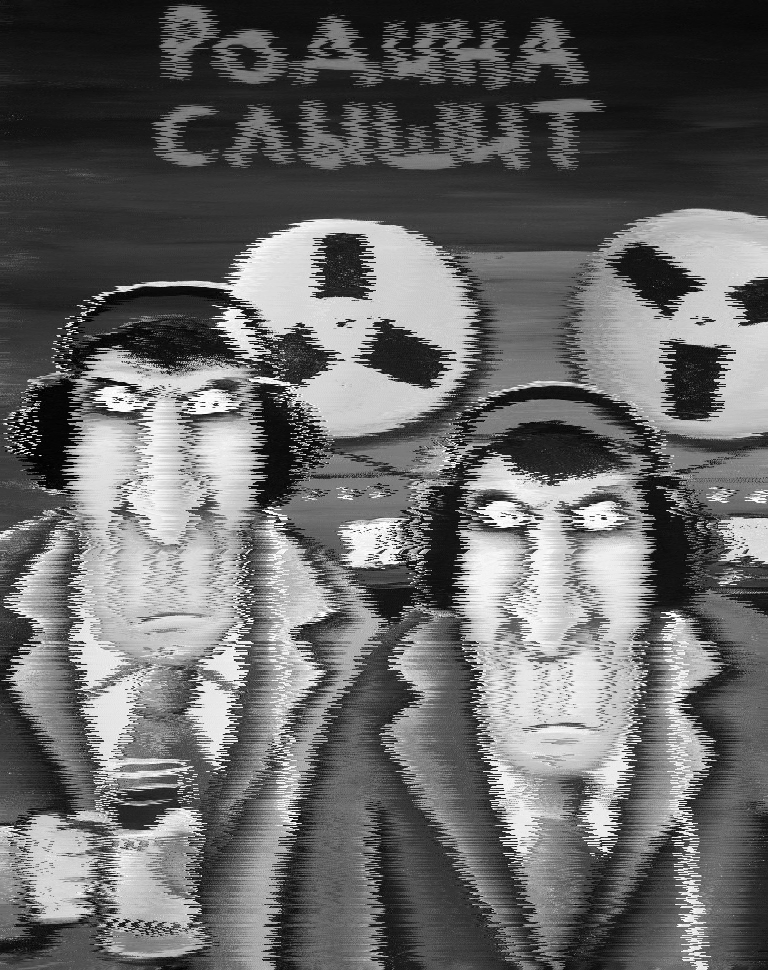
\includegraphics[height=0.8\textheight]{pic6.png}<1>
        \begin{itemize}
                \item<2-> Не позволяет анализировать DNS-запросы
                \begin{itemize}
                        \item<3-> Нарушает корпоративные стандарты безопасности
                        \item<4-> Мешает приложениям защиты отслеживать действия браузера
                        \item<5-> Создаёт видимость безопасности % конечно, есть серебряная пуля
                \end{itemize}
                \item<6-> Дополнительная нагрузка
                \item<7-> Цикл получения ответа неприемлимо долгий
        \end{itemize}
\end{frame}

\begin{frame}{Реакционизм. Гоcрегулирование}
        \only<1>{Картинка с самураем и флажками/нашивками РКН/FCC/etc}
        \begin{itemize}
                \item<2-> Давление UK ISPA % https://www.opennet.ru/opennews/art.shtml?num=51046
                \item<3-> Большинство «госблокировок» в мире основано на манипуляциях с DNS
                \item<4-> НСДИ РФ не совместима с DNSSEC % в принципе не намеренно
                \item<4-> НСДИ РФ не поддерживает защиту % а зря, буква "Б" в Роскомнадзор, ГРЧЦ, ЦМУ ССОП и НСДИ
        \end{itemize}
\end{frame}

\begin{frame}{Госрегулирование. НСДИ}
        \begin{itemize}
                \item Определена в законе 90-ФЗ от 01.05.2019
                \item Государственный публичный DNS
                \item Дублирует \textbf{.} (корень)
                \item Уменьшает ущерб от манипуляций с \textbf{\texttt{.RU}} \\
                {\small гипотетических, со стороны США в лице ICANN}
                \item НСДИ обслуживается ЦМУ ССОП
                \item Предоставляется в том числе AXFR
        \end{itemize}
\end{frame}

\begin{frame}{Безопасность заложенная в НСДИ}
        
\includegraphics[height=0.5\textheight,center]{travolta.png}<2->
\end{frame}

\begin{frame}{Многое осталось за кадром}
        \begin{itemize}
                \item EDNS(0) Padding, Cookies, etc
                \item Обслуживание DNS, DNSSEC, DoT/DoH
                \item Применение DNSSEC: DANE, etc
                \item Обзор серверов, включая \texttt{stub-ресолверы}
                \item Обзор клиентов и инструментов
                \item DNS Stamps (ссылки sdna://)
                \item \texttt{glibc} и \texttt{resolv.conf}
                \item Ampliphication attack, etc
                \item \textbf{...}
        \end{itemize}
\end{frame}

\begin{frame}{Вопросы}
        \center Перед докладом я многое освежил в памяти, многое не вошло в доклад
        \vskip1cm
        \center В любом случае пишите мне
        \vskip2cm
        \center{schors@gmail.com}
\end{frame}

%%% Всякая хрень
% https://dnscrypt.info/stamps-specifications  ссылки sdns://
% https://github.com/ameshkov/dnscrypt клиент dnscrypt


\nocite{*}
\setbeamertemplate{frametitle continuation}{}

\begin{frame}[t]{Ссылки. DNSCurve}
\printbibliography[keyword={dnscurve},notkeyword={en}]
\end{frame}

\begin{frame}[t]{Ссылки. DNSSEC}
\printbibliography[keyword={dnssec},notkeyword={en}]
\end{frame}

\begin{frame}[t]{Ссылки. DNSCrypt}
\printbibliography[keyword={dnscrypt},notkeyword={en}]
\end{frame}

\begin{frame}[t]{Ссылки. DoH/Dot}
\printbibliography[keyword={doh},notkeyword={en}]
\end{frame}

\begin{frame}[t]{Ссылки. Разное}
\printbibliography[keyword={extra},notkeyword={en}]
\end{frame}

\begin{frame}[t]{Ссылки. \LaTeX }
\printbibliography[keyword={latex},notkeyword={en}]
\end{frame}

\end{document}


